
\textbf{Observer le module de la transformée de Fourier. Quelle est la bande de fréquence utile pour le signal ?}
\begin{figure}[h]
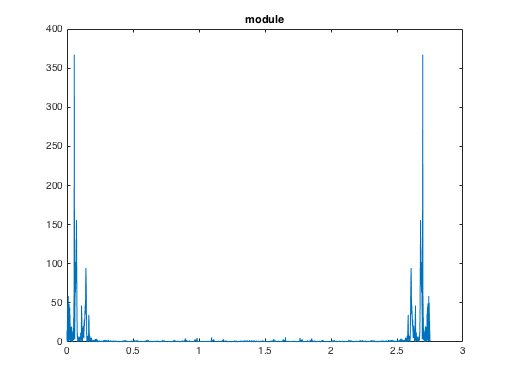
\includegraphics [width=.9\linewidth]{./img/module}
\caption{Module du signal issu de coucou.wav}
\end{figure}

La bande de fréquence utile pour le signal est [0 2.8]
\section{Filtre passe bas à réponse impulsionnelle finie}


\subsection{ Partie théorique}
Soit le filtre passe bas à réponse impulsionnelle finie :
y(k) = x(k)+x(k-1)+...+x(k-D)\\

Écrire ce filtre sous forme récursive.

\begin{math}
y(k) = x(k)+x(k-1)+...+x(k-D)\\
y(k-1) = x(k-1)+x(k-2)+...+x(k-(D+1))\\
y(k) = x(k)+y(k-1)-x(k-(D+1))\\
y(k) - y(k-1)= x(k)-x(k-(D+1))\\
Y(z) - z^{-1}Y(z)  = X(z)-z^{-(D+1)}X(z)\\
Y(z) (1- z^{-1}) = X(z)(1-z^{-(D+1)})\\
Y(z)=\frac{1-z^{-(D+1)}}{1- z^{-1}}X(z) \\
\end{math}

Fonction de transfert :\\
$H(z)=\frac{1-z^{-(D+1)}}{1- z^{-1}}$\\

Module : \\
$H(f)=\frac{1-e^{-2\pi jfTe(D+1)}}{1- e^{-2\pi jfTe}}\\
|H(f)|=\frac{|1-cos(2\pi jfTe(D+1))+j sin(2\pi jfTe(D+1))|}{|1-cos(2\pi jfTe)+j sin(2\pi jfTe)|}\\
|H(f)|=\frac{(1-cos(2\pi jfTe(D+1)))^{2}+ sin^{2}(2\pi jfTe(D+1))}{(1-cos(2\pi jfTe))^{2}+ sin^{2}(2\pi jfTe)}\\
|H(f)|=\frac{2-2cos(2\pi jfTe(D+1))}{2-2cos(2\pi jfTe)}\\
$

Représentation du module du filtre :\\
La représentation du module du filtre n'est pas envisageable avec le résultat obtenu à l'étape précédente, car lorsque $cos(2\pi jfTe)=1$ nous obtenons une forme indeterminée. Nous allons donc utiliser la règle de l'Hopital.\\
$\lim\limits_{z^{-1}\rightarrow 1}H(z)=\lim\limits_{z^{-1}\rightarrow 1} \frac{1-z^{-(D+1)}}{1- z^{-1}}\\
\lim\limits_{z^{-1}\rightarrow 1}H(z)=\frac{(D+1)z^{-D-2}}{z^{-2}}\\
\lim\limits_{z^{-1}\rightarrow 1}H(z)=D+1\\
$\\